% =====================================================================================================================
% research_monograph/manuscript_npj/main.tex -- MANUSCRIPT FRAMEWORK for npj Computational Materials.
% Status: FRAMEWORK FOR HUMAN REVIEW, 2026-10-14. Under charter section 9 no AI agent may put claims in a manuscript
% without explicit human approval: every sentence below that states a result is a CANDIDATE, tagged with its evidence
% (\ev{...}; CLAIMS_USED.tsv) and marked AWAITING APPROVAL there. Nothing here is approved, submitted or public.
% Sealed or blind results (ATLAS campaign S2-S7, runs 0075-0077, C10_DIAGb; every electronic quantity of the amorphous
% aIO_*/aIWO_* cells) appear only as \sealed{...}. Do not fill them by inference from any figure, log or file name.
% Device data (four transfer curves) belong to the fabrication group; their use in a publication needs written
% permission (DECISIONS.md N01).
% Build (from this folder): bash build.sh  ->  build/main.pdf
% Checks: python3 -I check_manuscript.py (claim IDs, facts, placeholders, forbidden phrases).
% =====================================================================================================================
\documentclass[11pt]{article}
% ms_preamble.tex -- packages and macros for the npj Computational Materials manuscript framework.
% Notation macros follow report_latex_full/preamble.tex. ASCII only. The journal's own template is NOT used here:
% its current requirements must be checked against the journal's guide for authors before submission (DECISIONS.md, N36).
\usepackage[T1]{fontenc}
\usepackage[utf8]{inputenc}
\usepackage[a4paper,margin=2.5cm]{geometry}
\usepackage{setspace}
\onehalfspacing
\usepackage[expansion=false]{microtype}
\setlength{\emergencystretch}{3em}
\usepackage{amsmath}
\usepackage{newtxtext,newtxmath}
\usepackage{graphicx}
\graphicspath{{../figures/}{../../qe_workflow/analysis_2026-10-13_full/figures/}%
  {../../qe_workflow/analysis_2026-10-13_full/bands_masses/figures/}}
\usepackage{booktabs,array,tabularx}
\usepackage{caption}
\captionsetup{font=small,labelfont=bf,labelsep=period}
\usepackage{enumitem}
\setlist{itemsep=2pt,topsep=4pt}
\usepackage[dvipsnames]{xcolor}
\usepackage[numbers,sort&compress]{natbib}
\usepackage[hidelinks]{hyperref}
\usepackage[capitalise,noabbrev]{cleveref}

% ---------------- notation (as in the report) ----------------
\DeclareRobustCommand{\file}[1]{\texttt{\detokenize{#1}}}
\newcommand{\prov}[1]{\textsc{\MakeLowercase{#1}}}
\newcommand{\InO}{In$_2$O$_3$}
\newcommand{\HfO}{HfO$_2$}
\newcommand{\AlO}{Al$_2$O$_3$}
\newcommand{\Vth}{V_{\mathrm{th}}}
\newcommand{\Vthcc}{V_{\mathrm{th,cc}}}
\newcommand{\Eg}{E_{\mathrm{g}}}
\newcommand{\dEc}{\Delta E_{\mathrm{c}}}
\newcommand{\dEv}{\Delta E_{\mathrm{v}}}
\newcommand{\tHH}{t_{\mathrm{HH}}}
\newcommand{\mzero}{m_0}
\newcommand{\PRn}{\mathrm{PR}_n}
\newcommand{\cmcu}{\ensuremath{\,\mathrm{cm}^{-3}}}

% ---------------- framework macros ----------------
% \ev{IDs}: evidence tag of a sentence: manuscript claim (MS-nn, CLAIMS_USED.tsv), ledger claim (C0nn), fact (Fnnn)
% or monograph section. Printed small and grey for review; \evfalse in the next line hides every tag.
\newif\ifev \evtrue
\newcommand{\ev}[1]{\ifev\textsf{\scriptsize\color{gray}[#1]}\fi}
% \pending{Nnn}{KIND: text}: a gap that waits for a result, a decision, a check or a citation (DECISIONS.md).
\newcommand{\pending}[2]{\textbf{[#1~#2]}}
% \sealed{text}: a result that is sealed or blind under the release protocol (decision D-43). Never fill by inference.
\newcommand{\sealed}[1]{\textbf{[SEALED: #1]}}
% intent paragraph of a section that cannot be written yet
\newenvironment{intent}{\par\noindent\textit{Intent.}\ }{\par\medskip}
\DeclareRobustCommand{\cell}[1]{\texttt{\detokenize{#1}}}


% Working title (NOT approved, N32): "Confinement, non-parabolicity and resonant tungsten donors in ultrathin In2O3:
% first-principles inputs for a shared-parameter transistor model, tested under pre-registration"
\title{\pending{N32}{TITLE: written after the release decision on the sealed results}}
\author{\pending{N34}{DECISION: authors, order and affiliations, agreed with the fabrication group}}
\date{Manuscript framework, 14 October 2026 -- not for circulation}

\begin{document}
\maketitle

\begin{abstract}
\noindent\textit{Candidate abstract (not approved; every clause is a claim in CLAIMS\_USED.tsv).}
Device models of ultrathin oxide-semiconductor transistors take the thickness dependence of the band edges, the
electron mass and the donor behaviour from first-principles calculations, usually one input at a time. We compute these
inputs for crystalline In$_2$O$_3$ films of 0.46--1.96~nm and for W-doped cells with PAW-PBE, and test their transfer to
a device model whose parameters are shared across thickness. The gap opening of the films, 0.34~eV at 1.96~nm and
0.90~eV at 0.93~nm, lies mostly in the conduction band, and the increase of the in-plane electron mass with
confinement is consistent, with no fitted quantity, with the bulk Kane non-parabolicity at the energy of the confined
subband (within 1\,\% at 1.96~nm and 10\,\% at 0.93~nm); to that accuracy the mass law and the band-shift law are one
input, not two. Substitutional W is a resonant donor whose
5d-rich state lies 1.2--1.8~eV above the conduction-band minimum at the computed filling, and W raises the energy of a
neutral oxygen vacancy far from it by 0.73~eV in the degenerate cell. Transferred rigidly to the device threshold, the
computed conduction-band shift accounts for 44\,\% of the measured difference between 2.0 and 13.2~nm channels but implies
a 0.2~V change between 2.0 and 6.3~nm that the measurement does not show, the same direction and size as every failed
out-of-sample threshold prediction at 6.3~nm. \pending{N33}{TEXT: sentence on the shared-parameter campaign and the
amorphous W read-out, only after release (D-43)}. All tests were registered before their outcomes; we report the
unresolved and failed ones with the same weight as the others.
\end{abstract}

\section*{Status of this framework}
This file fixes the structure, the candidate wording of every supported result and the place of every result that is
still sealed, blind or pending. It is not a draft for submission. Every result sentence carries an evidence tag
(\ev{MS-nn}, resolved in \file{CLAIMS_USED.tsv}; ledger claims \ev{C0nn}; facts \ev{Fnnn} of
\file{research_monograph/evidence/FACT_REGISTRY.tsv}); the tags can be hidden with \verb|\evfalse| in the preamble.
Each claim needs the approval of the research owner before it can stay (charter section 9). Open decisions, checks and
missing results are numbered N01--N45 in \file{DECISIONS.md}. The journal's current requirements (length, display
items, reference style, statements) were not checked in this session (N36).

% =====================================================================================================================
\section{Introduction}
\label{sec:intro}

Ultrathin \InO{}-based channels are candidates for transistors made within back-end-of-line thermal budgets
\citep{Januar2026}, and atomic-layer-deposited \InO{} channels as thin as 0.7~nm still switch off \citep{Si2021}.
Indium-based amorphous oxides are attractive because their conduction band is built from spherically symmetric metal s
orbitals, which tolerate disorder \citep{Nomura2004,Kamiya2010}. A few per cent of W in amorphous In--W--O channels
gives high mobility and improved stability at low process temperature \citep{Kizu2014}, and the stability of W-doped
\InO{} (IWO) transistors depends on the channel thickness \citep{Kim2024}. The fabrication group of this project
reported transfer curves of an IWO series with channels from 2.0 to 31.8~nm, analysed with an analytic device model and
first-principles calculations \citep{Januar2026}; under a registered extraction, the threshold voltage of these devices
rises by 0.58~V from 13.2 to 2.0~nm \ev{C002}.

A device model can reproduce such a series with per-film parameters, and then agreement is not evidence. The question is
which parts of the thickness dependence the material inputs computed from first principles can carry when the model
parameters are shared across all thicknesses, and which they cannot. Three inputs matter: the shift of the
conduction-band edge with thickness, which moves the threshold through the electron affinity; the electron mass, which
sets the density of states and the mobility; and the behaviour of the dopant, which sets the free-carrier density.
Each is usually computed and used on its own.

Here we compute all three for crystalline \InO{} films and W-doped cells with one set of numerical settings, show that
two of them are not independent, and test their transfer to a device model with shared parameters. The tests, including
an exploratory read-out of amorphous W-doped films, were registered before their outcomes were known
(\cref{sec:methods-registration}); the device comparisons are retrospective, because all four devices had been seen.
\pending{N35}{TEXT: final paragraph listing the hypotheses actually reported, after release}

% =====================================================================================================================
\section{Results}
\label{sec:results}

\subsection{Confinement of crystalline \texorpdfstring{\InO}{In2O3} films}
\label{sec:r-confinement}

Relaxed, hydrogen-passivated \InO{}(001) films with H--H thicknesses $\tHH$ of 0.930 and 1.962~nm have PBE gaps of
1.789 and 1.224~eV, 0.900 and 0.335~eV above the bulk gap of 0.889~eV \ev{C020; F002, F010d, F011d}. The two
thinnest films are not oxide films of the same kind: the 0.461~nm film relaxes to an In$_8$(OH)$_{24}$ layer
(gap 3.14~eV), and the 0.695~nm film is polar and was computed without a dipole correction, which leaves a
$\pm0.17$~eV uncertainty on its conduction-band shift \ev{C021; F016, F017, F018}. These two points are shown but are
excluded from the primary laws \ev{MS-01}.

Aligned to the bulk through the planar-averaged potential, the conduction-band minimum rises by 0.281~eV at 1.962~nm
and 0.848~eV at 0.930~nm, while the valence-band maximum falls by only 0.054 and 0.052~eV \ev{F014, F015}. The opening is
therefore mostly in the conduction band (84 and 94\,\%). Single-band envelope theory with the heavy, degenerate valence
band of \InO{} \ev{C040}, using the same confining wave vector for both bands and the non-parabolic conduction band,
reproduces the 0.930~nm partition (valence shift at most 0.061~eV, share 0.93); at 1.962~nm it predicts at most
0.016~eV, and the computed valence shift exceeds this by about 38~meV, more than the 5~meV spread between two
alignment routes and the 8~meV flatness of the interior potential. This excess is unexplained; a systematic error
common to both alignment routes is not excluded \ev{MS-02}. Between 1 and
2~nm the conduction-band shift scales as $t^{-1.48}$, below the exponent of 1.62 that the bulk Kane band predicts for a
box whose width is proportional to $t$ \ev{MS-03; F022, F028}. Hybrid-functional (HSE06) checks scale the PBE gap opening
by 1.06--1.11 \ev{C020; F030}. \Cref{fig:levels} shows the series.

\begin{figure}[htbp]\centering
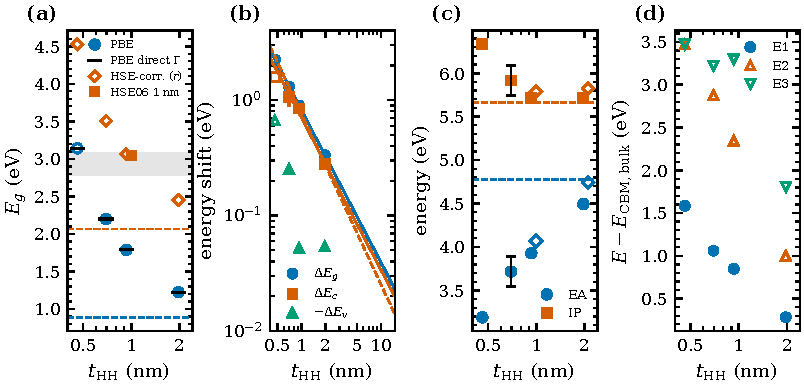
\includegraphics[width=\linewidth]{BM7_gaps_edges_laws}
\caption{\textbf{Gaps and band edges of crystalline \InO{}(001) films against H--H thickness (PAW-PBE).}
(a) Gap: PBE (circles; open: 0.461~nm), HSE-corrected (diamonds), computed HSE06 at 1~nm (square); dashed: bulk PBE
and HSE06; grey band: experimental fundamental gap $2.93\pm0.15$~eV \citep{King2009}. (b) Gap opening, conduction-band
shift and valence-band shift (log--log) with the fitted laws; bar at 0.695~nm: vacuum-reference sensitivity.
(c) Electron affinity and ionisation potential of the pure and W-doped films. (d) Conduction levels at $\Gamma$.
Panel content to be confirmed for the main text (\file{FIGURE_PLAN.tsv}, Fig.~1).}
\label{fig:levels}
\end{figure}

\subsection{The mass increase follows from the band shift}
\label{sec:r-mass}

The bulk conduction band has a band-edge mass of $0.154\,m_0$, isotropic within 0.2\,\%, and a Kane non-parabolicity
$\alpha = 0.58$~eV$^{-1}$ \ev{C039; F004, F005}; both are below the measured band-edge mass of
$0.208\pm0.006\,m_0$ \citep{Stokey2021}, as expected for PBE. The in-plane band-edge masses of the films rise to 0.203,
0.279, 0.337 and $0.443\,m_0$ at 1.962, 0.930, 0.695 and 0.461~nm \ev{C039; F026a--F026d}. For a Kane band, a subband
at energy $E_1$ above the bulk minimum has the in-plane band-edge mass $m_b(1+2\alpha E_1)$. With the computed $\dEc$ in
place of $E_1$ and the bulk $m_b$ and $\alpha$, this relation reproduces the computed mass within 1\,\% at 1.962~nm and
overestimates it by 10\,\% at 0.930~nm, with no fitted quantity (\cref{fig:mass}) \ev{MS-04; F027}; the two thinner
films agree within 2\,\% but do not test the relation (one lies far outside the fitted energy window, the other carries
a $\pm9$\,\% uncertainty from its polar field). To this accuracy the mass increase at 2~nm is the bulk non-parabolicity
probed at the subband energy, and a device model that takes both a mass law and a band-shift law from these films
carries one independent first-principles input, not two \ev{MS-04}.

The valence band has no single band-edge mass: its top is three-fold degenerate at $\Gamma$ with a camel back 4.4~meV
high, and its effective density of states at 300~K, $1.6$--$2.7\times10^{21}$\cmcu{}, is defined only as a band
integral \ev{C040; F060, F062}.

\begin{figure}[htbp]\centering
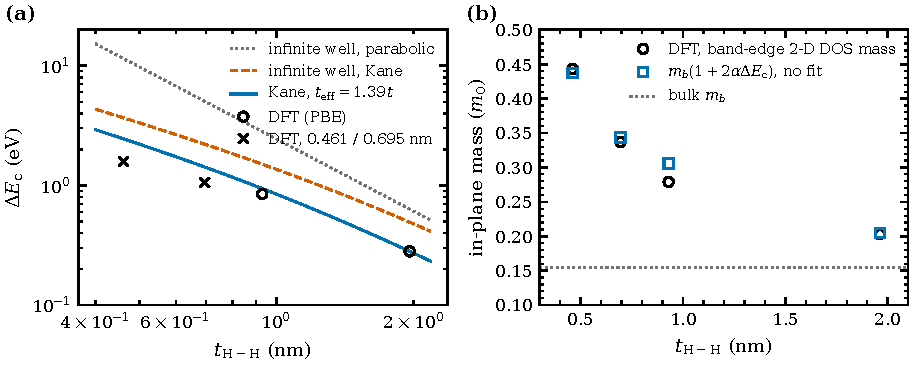
\includegraphics[width=\linewidth]{mono_confinement_models}
\caption{\textbf{Computed films against confinement models (PBE).} (a) Conduction-band shift against H--H thickness:
computed (circles; crosses: the 0.461~nm In$_8$(OH)$_{24}$ layer and the polar 0.695~nm film), infinite parabolic well
with the bulk mass (dotted), with the bulk Kane non-parabolicity (dashed), Kane band with box width $1.39\,\tHH$
(solid). (b) In-plane band-edge mass: computed (circles) against $m_b(1+2\alpha\dEc)$ with the computed $\dEc$ and no
fitted quantity (squares); dotted: bulk $m_b$.}
\label{fig:mass}
\end{figure}

\subsection{W is a resonant donor in crystalline \texorpdfstring{\InO}{In2O3}}
\label{sec:r-w}

W substitutes preferentially on the 24d cation site (by 0.258~eV over 8b in 80-atom cells) \ev{C022; F040}. In bulk
cells with 3.1\,\% W and in films with W on a central 24d site, the state with the largest W-5d weight is a resonance
1.22 (0.93~nm film), 1.34 (1.96~nm film) and 1.76--1.80~eV (bulk) above the host conduction-band minimum, and the Fermi
level lies 1.2--1.8~eV inside the host conduction band (\cref{fig:w}) \ev{C022; F042, F043}. W thus donates its electrons
to the host conduction band, which it makes 5\,\% heavier \ev{C039; F047}, as reported for Mo in \InO{}, where the
dopant states lie high in the conduction band and barely perturb its minimum \citep{Swallow2020}. The computed position
refers to the filling of the cell, $1.4$--$3.0\times10^{21}$ donated electrons per cm$^3$; whether the W level stays
above the band edge at device densities, two to three orders of magnitude lower, is inferred, not computed
\ev{MS-05; C022}. Spin-polarised calculations give W moments of 0.62 and 0.74~$\mu_{\mathrm{B}}$ (24d, 8b) that are likely artefacts of the
coarse $k$ sampling of a degenerate electron gas; we do not interpret them \ev{MS-06; F046}.

An earlier analysis of the same calculations placed the W level below the conduction band; this was a band-counting
error (the In data set includes the 4d shell and the W data set the 5s5p shells, so a W cell has one fewer occupied band
below the gap than an In cell) and is corrected here \ev{MS-07}. \pending{N41}{DECISION: whether the correction is
reported in the paper or only in the Supplementary Information}

\begin{figure}[htbp]\centering
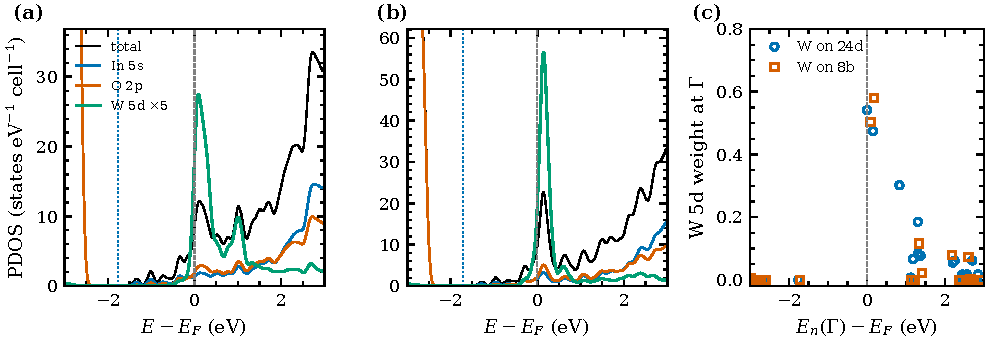
\includegraphics[width=\linewidth]{fig09_iwo_bulk_pdos}
\caption{\textbf{W in bulk \InO{} (80-atom cells, PBE).} (a) W on 24d, (b) W on 8b: total density of states and
projections on In 5s, O 2p and W 5d (W 5d $\times5$) against $E-E_F$; dashed: $E_F$; dotted: bottom of the host
conduction band at $\Gamma$. (c) W-5d weight of each state at $\Gamma$ against energy. The film cells are shown in
Supplementary Fig.~S5.}
\label{fig:w}
\end{figure}

\subsection{Oxygen vacancies near and far from W}
\label{sec:r-vacancy}

We tested whether W raises the energy of a neutral oxygen vacancy (registered hypothesis H-L). In 80-atom cells
(PBE, fixed cell, relaxed on a $3\times3\times3$ grid and evaluated also on $4\times4\times4$), a vacancy far from W costs
$\Delta E_{\mathrm{dop}} = +0.726$ (k3) and $+0.723$~eV (k4) more than a vacancy in pure \InO{}; this difference passes
its registered threshold of $+0.05$~eV and changes by only 3.4~meV between the two grids \ev{C038; F051}. A vacancy next to W costs a
further $+0.558$ (k3) and $+0.532$~eV (k4); both exceed the registered $+0.3$~eV, but the grid change of $-25.7$~meV
exceeds the registered 10~meV limit, so its significance is unresolved \ev{C038; F050}. The registered spin
sensitivity was not run, so the overall verdict of H-L is \prov{unresolved} (\cref{fig:hl}) \ev{MS-08; C038}. Both
differences include the filling of a conduction band already occupied to 1.7~eV above its bottom; they are not formation
energies at a device Fermi level \ev{MS-08}. \pending{N16}{RESULT: spin sensitivity A20(i), if run}

\begin{figure}[htbp]\centering
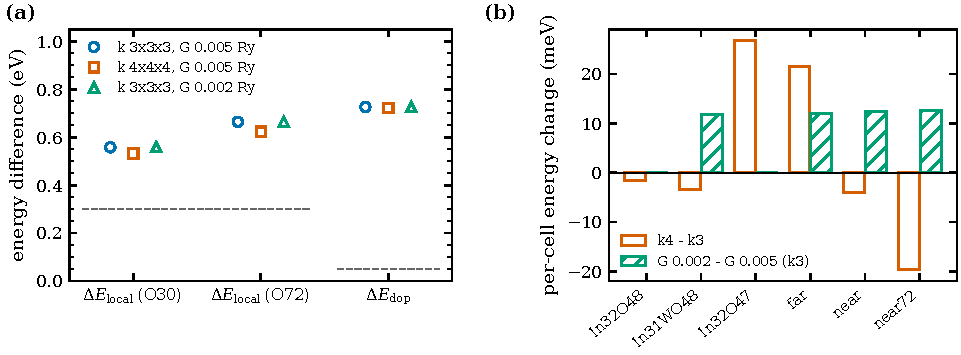
\includegraphics[width=0.95\linewidth]{fig11_hl_vacancy}
\caption{\textbf{Registered oxygen-vacancy test H-L.} (a) $\Delta E_{\mathrm{local}}$ for the registered near site
and a sensitivity site, and $\Delta E_{\mathrm{dop}}$, on two $k$ grids and two smearing widths; dashed: registered
thresholds. (b) Per-cell total-energy changes between the grids and widths.}
\label{fig:hl}
\end{figure}

\subsection{What the computed shift implies for the device threshold}
\label{sec:r-device}

The four devices of the series (one per thickness, $V_{\mathrm{D}} = 0.7$~V) have constant-current thresholds of
0.662, 0.644 and 0.083~V at 2.0, 6.3 and 13.2~nm under the registered extraction \ev{C002; F101--F103}.
\pending{N01}{DECISION: permission of the fabrication group to show and publish these data}. The fitted conduction-band
shift differs by 0.257~eV between 2.0 and 13.2~nm for every fit option; transferred rigidly to the threshold, it would
account for 44\,\% of the measured difference of 0.579~V \ev{MS-09}. Between 2.0 and 6.3~nm, the same shift implies a
threshold change of $-0.21$ to $-0.22$~V against a measured $-0.018$~V (\cref{fig:threshold}) \ev{MS-09}. Earlier
device models calibrated per film reproduce every threshold by construction \ev{C013}, and all three out-of-sample
predictions of the 6.3~nm threshold missed, by $-0.29$, $-0.37$ and $-0.23$~V \ev{C014}: the same direction and size as
the rigid transfer. The comparison does not identify a cause; from transfer curves alone the gate work function, the
bulk affinity, a uniform fixed charge and the confinement shift act as one number per film \ev{C018}, and the candidate
explanations (device-to-device spread, a thickness error, a different process history of the 6.3~nm device, a
non-monotonic film property) cannot be separated with one device per thickness \ev{MS-10}.

\begin{figure}[htbp]\centering
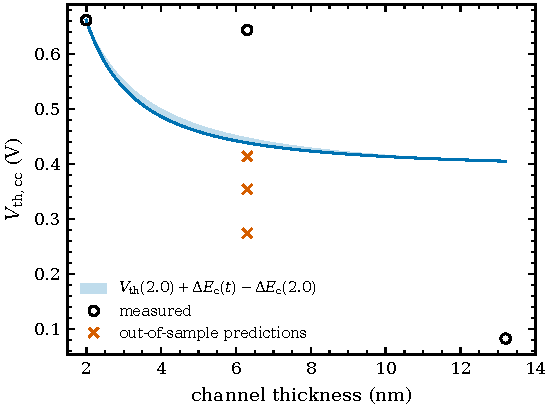
\includegraphics[width=0.62\linewidth]{mono_threshold_vs_dft}
\caption{\textbf{Measured thresholds against the computed band shift.} Circles: measured constant-current thresholds.
Band: $\Vth(2.0)+\dEc(t)-\dEc(2.0)$ over the fit options of the confinement law; line: two-parameter fit. Crosses: the
three failed out-of-sample predictions at 6.3~nm. A rigid transfer of the affinity shift; an illustration, not a model
run. Requires the fabrication group's permission (N01).}
\label{fig:threshold}
\end{figure}

\subsection{Shared-parameter device model}
\label{sec:r-shared}
\begin{intent}
Report the registered shared-parameter campaign as registered: the stage-1 checks already seen (marked as seen before
the register's revision 2), the confinement-off and affinity-only tests, the shared calibration as calibration, its
identifiability analysis and the retrospective leave-one-film-out folds. State failures as failures; no per-film rescue
parameters. Include the density-of-states convention sensitivity at 2~nm (142~mV), which is a model-side sensitivity
of about a third to two thirds of the 6.3~nm misses \ev{MS-11}.
\end{intent}
\sealed{ATLAS campaign C10 stages S2--S7, runs 0075--0077 and C10\_DIAGb; release by the D-43 protocol only}

\subsection{Amorphous W-doped films}
\label{sec:r-amorphous}

The amorphous cells were generated by melt-quench molecular dynamics with a machine-learned interatomic potential
(MACE-MPA-0 \citep{Batatia2022,Batatia2023}) and relaxed with PBE. The registered force check of the potential failed
for the W first shell, so the generated structures serve only as starting points for the DFT relaxation and are not
validated amorphous models \ev{C037; F070}. Two numerical controls passed: the forces of a relaxed cell change by at most
$2.4\times10^{-4}$~Ry/bohr between Marzari--Vanderbilt and Gaussian smearing \ev{C034; F071}, and splitting a species
label for the GPU route leaves energies and forces unchanged to $10^{-8}$~Ry and $3\times10^{-8}$~Ry/bohr
\ev{C035; F072}. One 0.8~nm relaxation did not converge and was not reproducible on restart with identical settings
\ev{C036; F073}.

Two properties of the registered read-out follow from its frozen rules alone, without any electronic result. First, its
absolute participation-ratio thresholds (localised if $\PRn \le 0.05$) correspond to different support sizes in cells
of different size: a state spread evenly over W and its six first-shell O atoms is localised in the 0.7, 0.8 and 2.0~nm
cells but intermediate in the bulk and 1.0~nm cells \ev{MS-12}. Second, the exploratory thickness test (H-N) cannot
return a crossover or a no-crossover verdict, because its 2.0~nm endpoint is unresolved in every branch \ev{MS-13}.
\sealed{per-cell classes and controls of the amorphous W cells (H-G, H-K, H-N); release by the D-43 protocol only}

% =====================================================================================================================
\section{Discussion}
\label{sec:discussion}

\textit{Candidate discussion points (not approved).}
\begin{enumerate}
\item The first-principles inputs of a confinement-aware device model of \InO{} are fewer than they appear: the mass law
follows from the band-shift law through the bulk non-parabolicity \ev{MS-04}. A model that fits both has one
independent input; a model that varies them independently can over-fit.
\item W behaves in crystalline \InO{} as a resonant donor, consistent with resonant doping by Mo \citep{Swallow2020}; we
did not find a peer-reviewed first-principles study of W in \InO{} to compare with \ev{MS-05}. At device densities the
position of the W level, polaron formation and compensation are not computed. The difference between full activation
($6\times10^{20}$ to $1.8\times10^{21}$\cmcu{} at 2\,\% W, one to three electrons per W) and the effective donor density of the calibrated device model
($2.5\times10^{17}$\cmcu{} for the thinnest films, rising to $1.8\times10^{18}$\cmcu{} at 31.8~nm) must come from compensation, inactive donors or both \ev{MS-14; C016}.
\item The computed band shift explains a substantial part of the threshold step between 2.0 and 13.2~nm, but its
monotonic thickness dependence is inconsistent with the 6.3~nm device \ev{MS-09}. With one device per thickness this is
the dominant unexplained feature of the data, and it cannot be resolved by calculation alone.
\item Registering the tests before their outcomes exposed design properties of the read-out (size-dependent thresholds,
an unreachable crossover verdict) before any blind result was opened \ev{MS-12, MS-13}. \pending{N30}{RESULT: the
scorecard of every registered prediction}
\item Measurements that would separate the inputs: flat-band voltage against thickness from capacitance--voltage curves,
the optical gap against thickness, photoemission band offsets, several devices per thickness and a drain-bias series
of the off-state floor \ev{MS-15}.
\end{enumerate}
\begin{intent}
Limits to state: PBE without $+U$ or hybrid relaxation; crystalline films against amorphous or nanocrystalline channels;
cells far more heavily doped than the devices; one device per thickness and retrospective device comparisons;
machine-learned starting structures that failed their force check.
\end{intent}

% =====================================================================================================================
\section{Methods}
\label{sec:methods}

\subsection{First-principles calculations}
\label{sec:methods-dft}
Quantum ESPRESSO 7.5 (CPU) and the NVIDIA GPU build 7.3.1 \citep{Giannozzi2009,Giannozzi2017,NvidiaQE}; PBE
\citep{Perdew1996}; PAW data sets of pslibrary 1.0.0 \citep{Bloechl1994,DalCorso2014} with In 4d and W 5s5p in the
valence; kinetic-energy cutoffs of 71~Ry (wavefunctions) and 568~Ry (density). Bulk bixbyite \InO{} relaxed to
$a = 10.306$~\AA{} \ev{F001}. Films: (001) slabs with hydrogen-passivated surfaces and 25~\AA{} of vacuum, relaxed at
fixed in-plane cell on $3\times3\times1$ grids; band edges aligned to the bulk by the two-step planar-average method
\citep{VandeWalle1987,Baldereschi1988}. Doped cells: Marzari--Vanderbilt smearing of 0.01~Ry \citep{Marzari1999};
L\"owdin projections \citep{Lowdin1950}. Masses: ten-point Kane fits near $\Gamma$ \citep{Kane1957}. Hybrid checks:
HSE06 \citep{Heyd2003,Krukau2006} with SG15 norm-conserving pseudopotentials \citep{Hamann2013,Schlipf2015} at 80~Ry
and the PBE geometry.
Vacancy cells (H-L): neutral 79/80-atom cells, Gaussian smearing 0.005~Ry, forces below $10^{-3}$~Ry/bohr.
\pending{N17}{CHECK: complete per-calculation settings table from the monograph (Ch.~13 and M04b) for the SI}

\subsection{Device simulation and extraction}
\label{sec:methods-tcad}
Silvaco ATLAS 5.28 \citep{AtlasManual}; drift--diffusion with tail and deep acceptor-like trap densities of states; gate stack 15~nm \HfO{} and 2~nm
\AlO{} ($C_{\mathrm{ox}} = 8.955\times10^{-7}$~F\,cm$^{-2}$) \ev{F100}. Thresholds by the registered constant-current
rule ($10^{-9}$~A\,$\mu$m$^{-1}$) \ev{C002}. \pending{N04}{CITATION: oxide band parameters, tunnelling masses and
capture cross-sections with page-exact sources}

\subsection{Registration}
\label{sec:methods-registration}
Hypotheses, read-out definitions and decision rules were frozen in a register (revision 2, 2026-10-10T18:33:13Z) before
the corresponding results were computed or opened; later amendments were logged with their time and the decision that
approved them. Results produced after the freeze are kept sealed until a release decision. \pending{N27}{CHECK:
external timestamp of the register (DOI or public tag)} \pending{N28}{DISCLOSURE: pre-release sight events, worded by
the register}

% =====================================================================================================================
\section*{Data availability}
\pending{N37}{TEXT: depends on the fabrication group's permission for the device data (N01); computed outputs and the
derived tables can be archived with a DOI (N38)}

\section*{Code availability}
\pending{N38}{TEXT: input generators, analysis scripts, read-out package with freeze tags, deck generator and scorer;
archive with a DOI}

\section*{Author contributions}
\pending{N34}{DECISION: author list and contributions}

\section*{Use of AI tools}
\begin{intent}
Describe the roles of the AI agents as practised: computational execution, analysis and record keeping by Claude Code,
independent review by Codex; every amendment needed a human decision; agreement between AI systems was not treated as
evidence; no AI agent placed a claim in the manuscript without approval.
\end{intent}
\pending{N39}{TEXT: statement in the wording the journal requires}

\section*{Competing interests and acknowledgements}
\pending{N40}{TEXT: competing interests; acknowledgements (CERN computing resources, funding)}

\bibliographystyle{unsrtnat}
\bibliography{../../report_latex_full/references,../../report_latex_full/bib/extra_DFT,../bib/monograph}

\end{document}
